\chapter{Evaluation and experiments}
\section{Single Quadrotor Control with Payload}
\begin{itemize}
    \item Recover from harsh and track position
    \item Follow trajectory
    \item Follow trajectory with disturbance
    \item Plots recovery: Recovery success rate for 10000 rollouts ofver time.
    \item Plots Traj: Trajectory following 3d, error over time for batch
    \item Plots Disturbance: Trajectory following with disturbance, error over time for batch

\end{itemize}
\begin{figure}
    \centering
    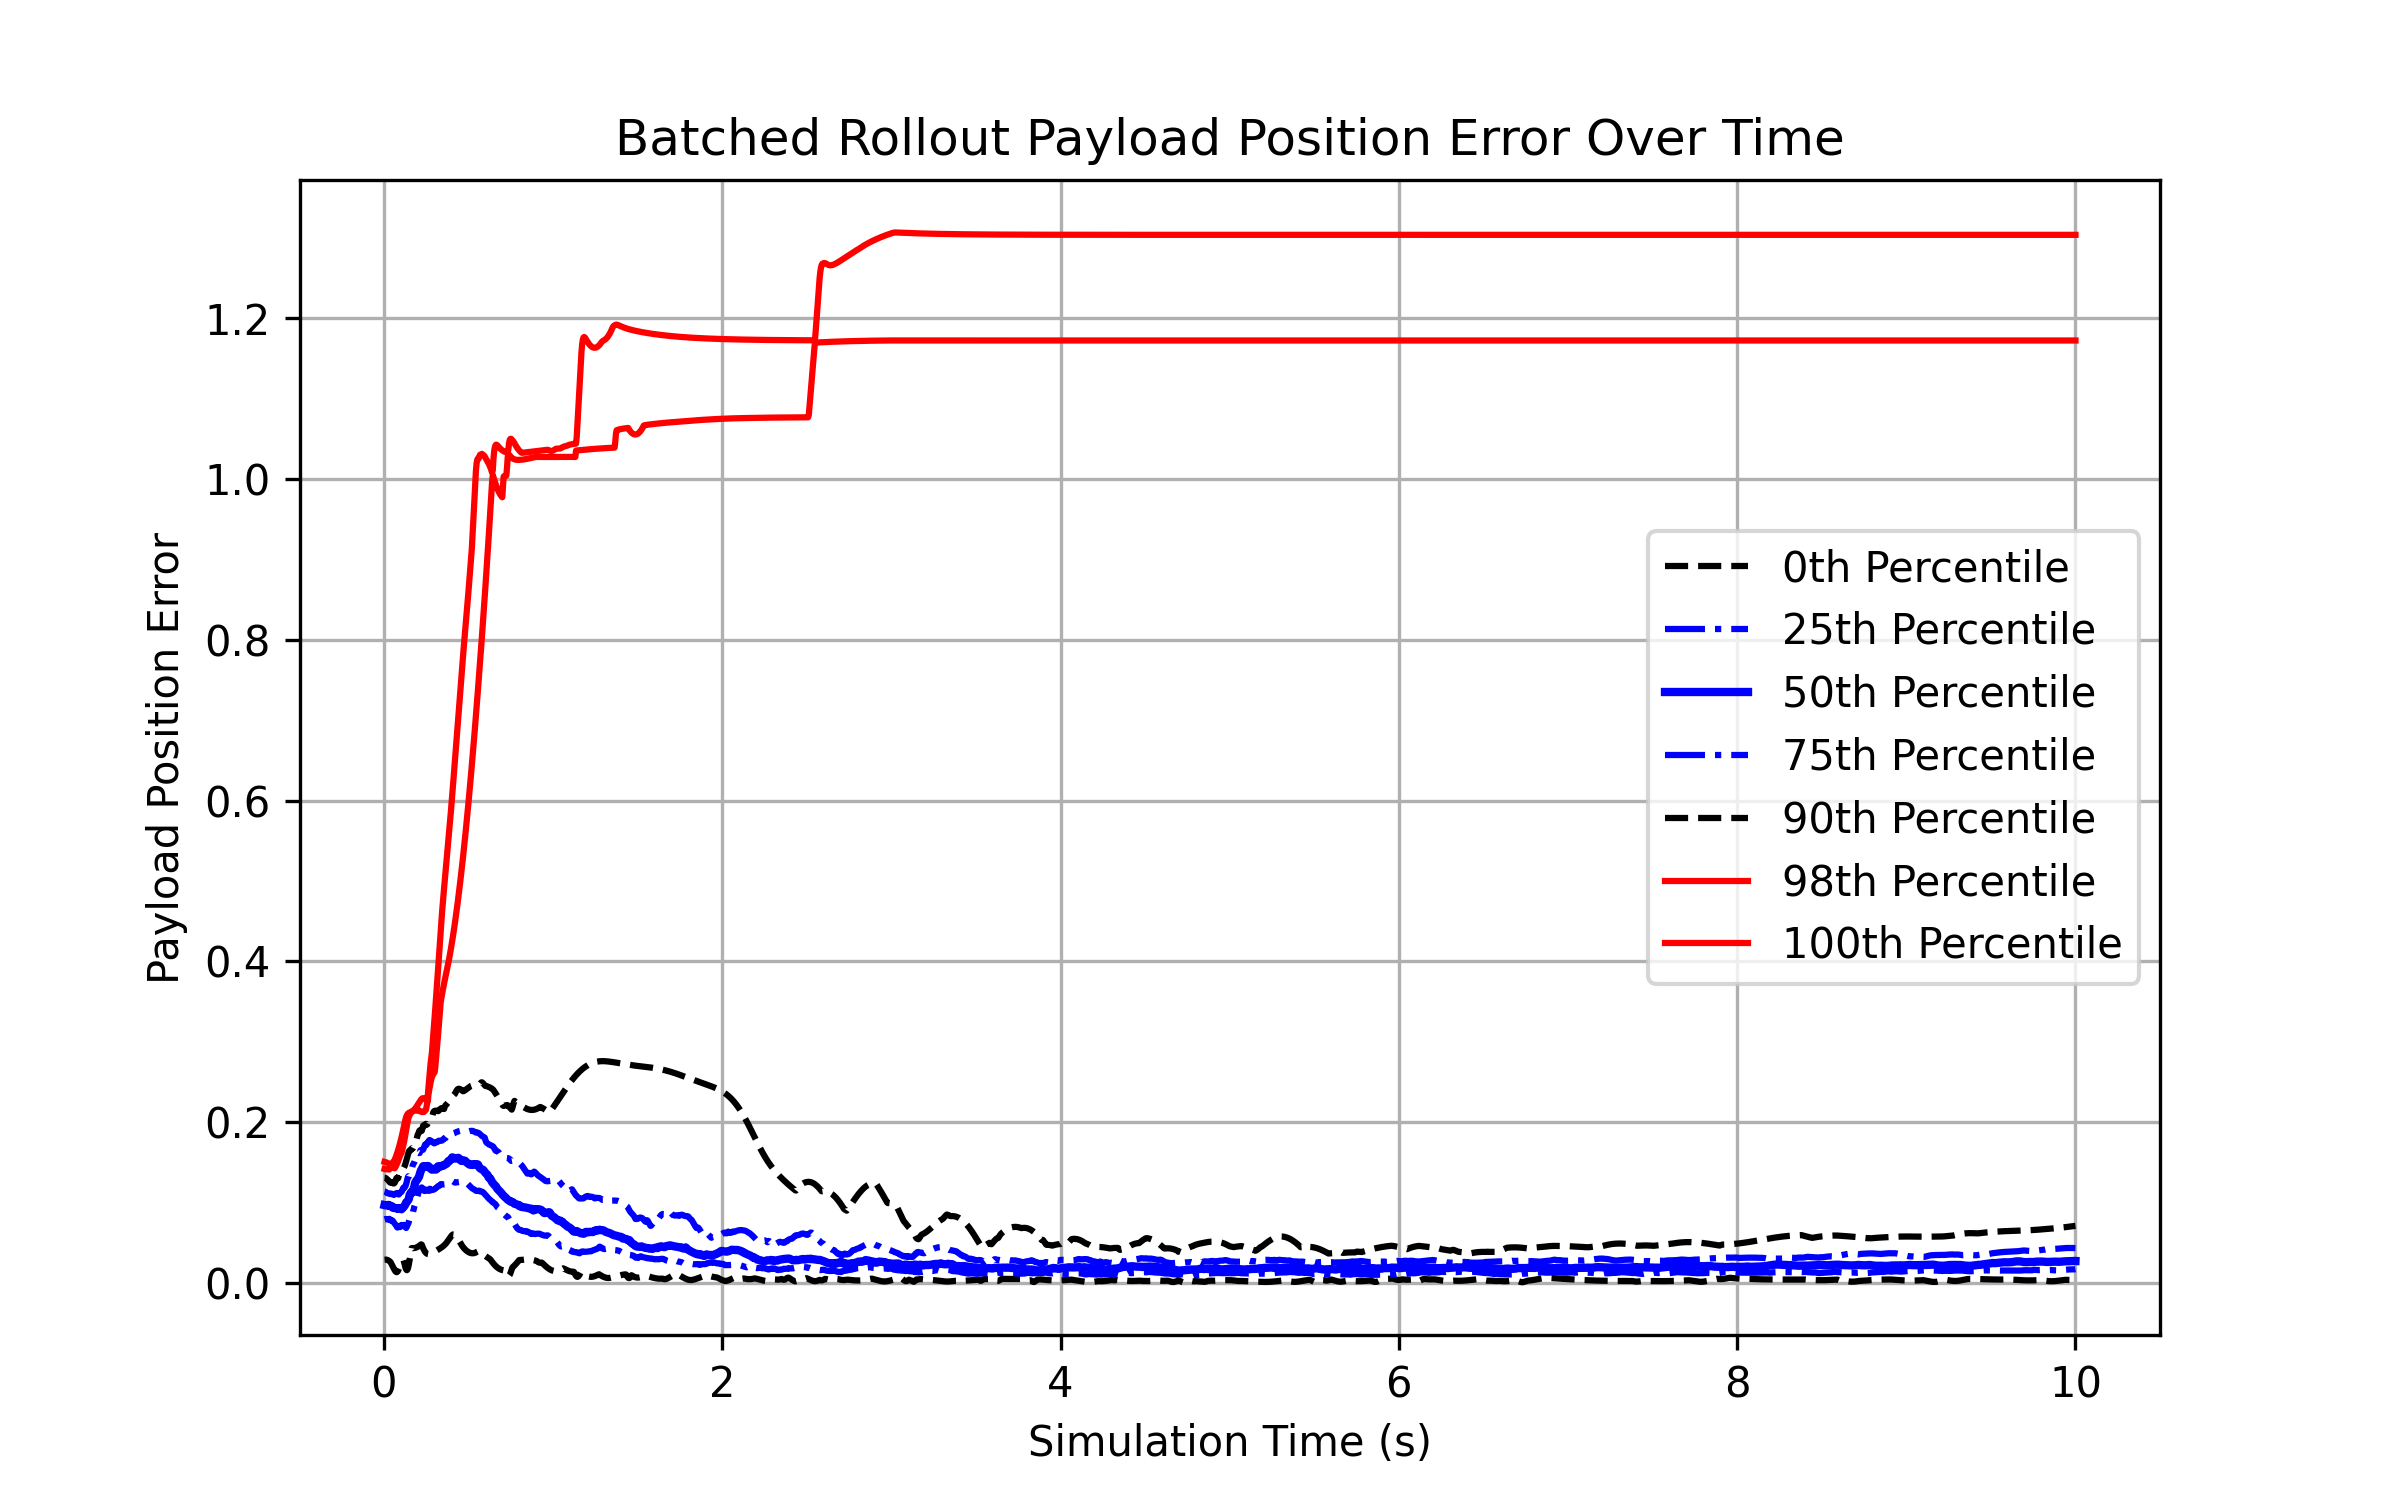
\includegraphics[width=\textwidth]{batch.png}
    \caption{Single quadrotor control with payload. The quadrotor is able to recover from harsh disturbances and track a desired position.}
    \label{fig:single_quadrotor_control}
\end{figure}
\begin{figure}
    \centering
    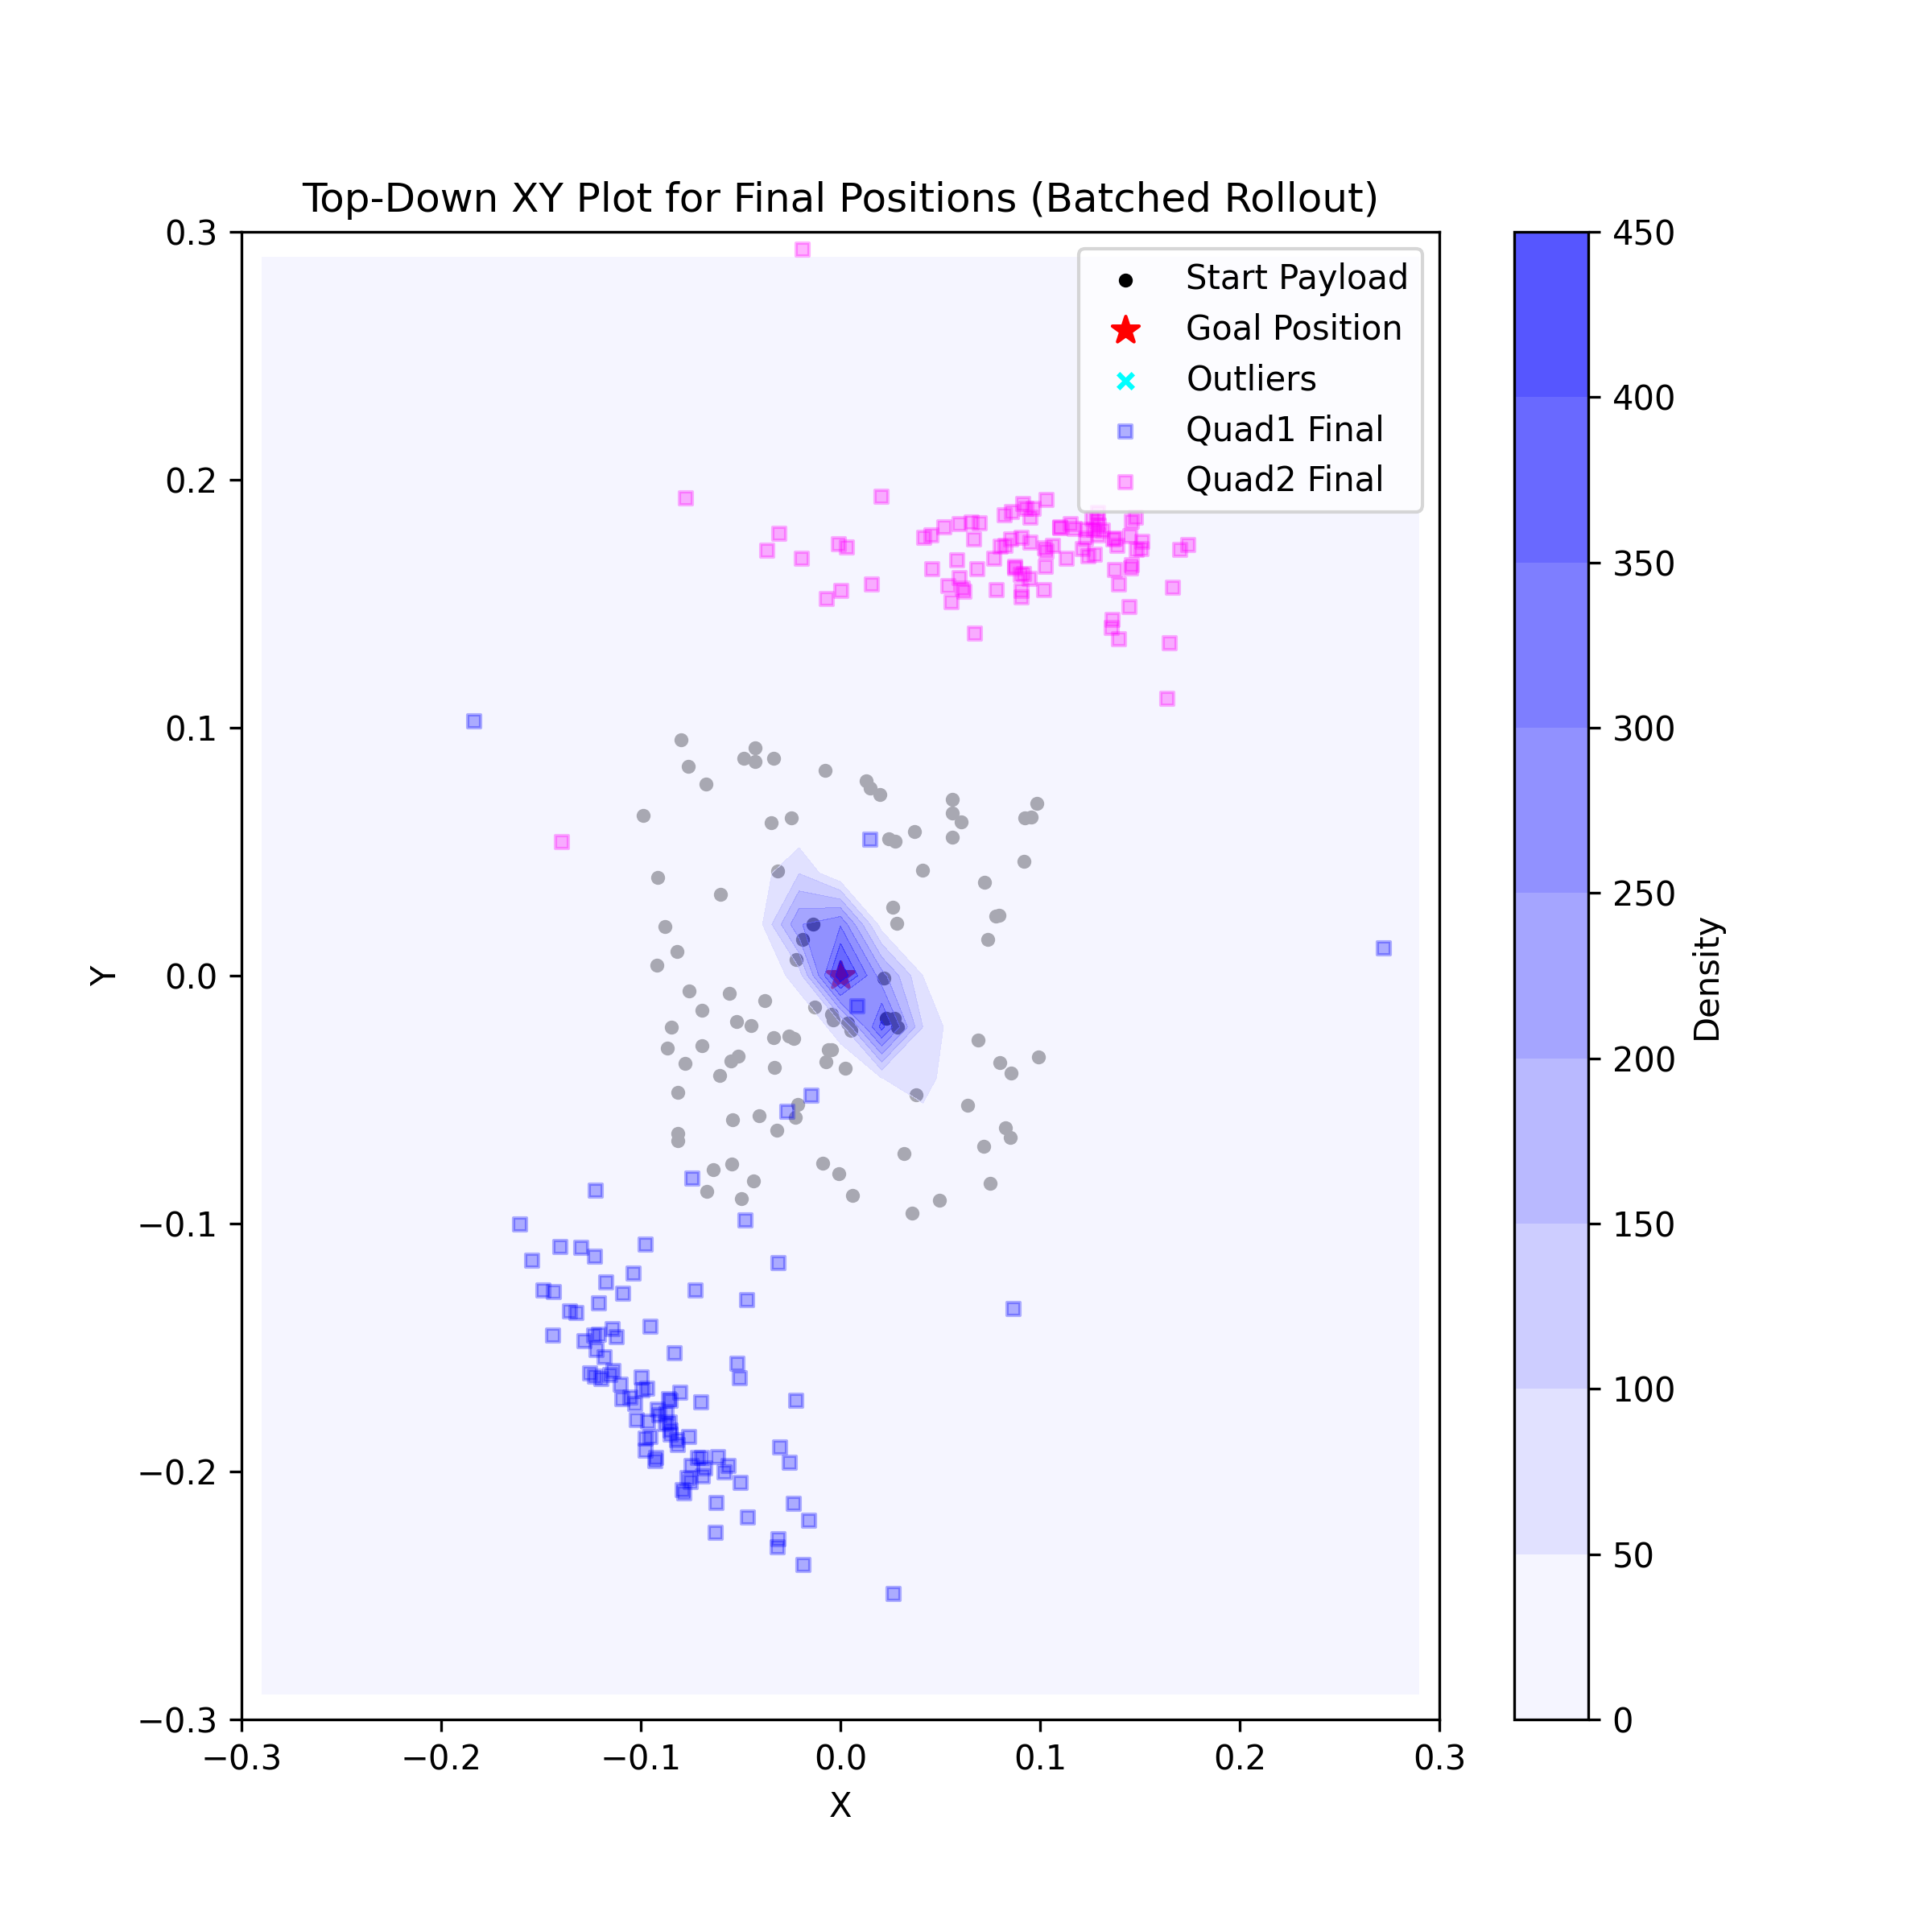
\includegraphics[width=\textwidth]{pos_recover.png}
    \caption{Single quadrotor control with payload. The quadrotor is able to recover from harsh disturbances and track a desired position.}
    \label{fig:single_quadrotor_control}
\end{figure}
\section{Multi Quadrotor Control with Payload}
\begin{itemize}
    \item Recover from harsh and track position
    \item Follow trajectory
    \item Follow trajectory with disturbance
    \item Plots recovery: Recovery success rate for 10000 rollouts ofver time.
    \item Plots Traj: Trajectory following 3d, error over time for batch
    \item Plots Disturbance: Trajectory following with disturbance, error over time for batch
\end{itemize}
% optional
\section{Comparison with classic control}
Compare with prev paper method \autocite{Wahba2024}
\begin{itemize}
    \item Plots Traj: Trajectory following 3d, error over time for batch
    \item Plots Disturbance: Trajectory following with disturbance, error over time for batch
    \item Plots ground start: Trajectory following with disturbance, error over time for batch
\end{itemize} 
\section{Sim-to-Real Transfer}
\begin{itemize}
    \item one and three quads
    \item Plots Traj: Trajectory following 3d,  error over time 
    \item Plots Disturbance: Position holding with disturbance
\end{itemize}


\section{Ablation Studies}
\begin{itemize}
    \item Ablation on reward design
    \item Ablation on training parameters
    \item Ablation on domain randomization